\documentclass[10.5pt]{article}

% Language setting
% Replace `english' with e.g. `spanish' to change the document language
\usepackage[english]{babel}

% Set page size and margins
% Replace `letterpaper' with`a4paper' for UK/EU standard size
\usepackage[letterpaper,top=2cm,bottom=3cm,left=2.5cm,right=2.5cm,marginparwidth=1.75cm]{geometry}

% Useful packages
\usepackage{tabularx}
\usepackage{amsmath}
\usepackage{multicol}
\usepackage{graphicx}
\usepackage{caption}
\usepackage{lipsum}
\usepackage[table]{xcolor}
\usepackage[colorlinks=true, allcolors=blue]{hyperref}
\newcommand\blfootnote[1]{%
  \begingroup
  \renewcommand\thefootnote{}\footnote{#1}%
  \addtocounter{footnote}{-1}%
  \endgroup
}
% Keywords command
\providecommand{\keywords}[1]
{
  \small	
  \textbf{\textit{Keywords --- }} #1
}


\title{\vspace{-2cm}\textbf{Toxic Comment Classification}}
\author{\small{\textit{Antonio Di Mauro  - 599785 - a.dimauro3@studenti.unipi.it - MSc in Artificial Intelligence}} \\ 
        \small{\textit{Domenico Tupputi - 585794 - d.tupputi@studenti.unipi.it - MSc in Artificial Intelligence}} \\ 
        \small{Human Languages Technologies, Academic Year: 2020/2021}}

\begin{document}
\newcolumntype{Y}{>{\centering\arraybackslash}X}

\begin{figure}
\centering

\includegraphics[width=0.3\textwidth]{uni.png}
\end{figure}
\maketitle

\begin{multicols*}{2}

\begin{abstract}
A large percentage of online comments on public domains are generally constructive, however a significant percentage are toxic in nature. In this article, we focus on the different approaches regarding the problem of the classification of toxic comments online.
This task is a research initiative founded by Jigsaw and Google (both part of Alphabet) who are working on tools, which use Natural Language Processing techniques, to help improve online conversation. \vspace{0.1cm} \\
\keywords{Natural Language Processing, Bert, Neural Network, Toxic comment classification, Deep learning, Preprocessing. }
\end{abstract}

\vspace{5pt}
\hrule
\vspace{6pt}
\begingroup
  \small
\textit{Permission to make digital or hard copies of all or part of this work for
personal or classroom use is granted without fee provided that copies
are not made or distributed for profit or commercial advantage and that
copies bear this notice and the full citation on the first page. Copyrights
for components of this work owned by others than the author(s) must
be honored. Abstracting with credit is permitted. To copy otherwise, or
republish, to post on servers or to redistribute to lists, requires prior specific
permission and/or a fee. Request permissions from permissions@acm.org.
HLT, 2019/20, University of Pisa, Italy
© 2021 Copyright held by the owner/author(s). Publication rights licensed
to ACM.
ACM ISBN 978-x-xxxx-xxxx-x/YY/MM. . . \$0.00
https://doi.org/10.1145/nnnnnnn.nnnnnnn}
\endgroup

\section{Introduction}
Keeping online conversations constructive and inclusive is a crucial task for platform providers.  Automatic classification of toxic comments, such  as hate speech, threats, and insults, can help in  keeping discussions fruitful. In addition, new regulations in certain European countries have been  established enforcing to delete illegal content in  less than 72 hours.

Active research on the topic deals with common challenges of natural language processing,  such as long-range dependencies or misspelled  and idiosyncratic words.

We will use a dataset of comments on Wikipedia talk  pages presented by Google Jigsaw during Kaggle’s Toxic Comment Classification Challenge \cite{competitiontoxic}. These sets include common difficulties in datasets  for the task: They are labeled based on different definitions; they include diverse language from  user comments; and they present a  multi-class and a multi-label classification task respectively.
In this work, we apply and compare different classifiers.  Each classifier, such as Logistic Regression, Multi-layer Perceptron, is meant to tackle specific challenges for text classification. We apply  the same classifiers to a dataset of validate our results.

Unfortunately for the problem, but fortunately for the Wikipedia community, toxic comments are rare. Just over 10\% of this dataset is labeled as toxic, but some of the subcategories are extremely rare making up less than 1\% of the data.

Because of this imbalance, accuracy is a practically useless metric for evaluating classifiers for this problem.


\end{multicols*}


\begin{center}
\centering % centering table
\begin{tabularx}{1\textwidth}{YYY}
\hline\hline %inserting double-line
Author & Models & AUC \vspace{0.1cm}\\
\hline \vspace{0.1cm}\\
HOON BENG \cite{logisticregressionsolution} &  Logistic Regression & 0.9741 \vspace{0.1cm}\\
AMIR ASHRAFF \cite{Forkofensemble_3_blend} & ensemble models & 0.98705 \vspace{0.1cm}\\
BOJAN TUNGUZ \cite{Bi-GRU-LSTMDualEmbedding}  & Bi-GRU-LSTM Dual Embedding & 0.98702 \vspace{0.1cm}\\ 
Jay Speidell \cite{jayspeidellToxicCommentClassification} & NB-SVM & 0.9747 \vspace{0.1cm}\\
SMU Data Science Review \cite{ToxicCommentOnelabel}  & SVM & 0.9725 \vspace{0.1cm}\\ 
Chun Ming Lee \cite{KaggleSOTA}  & Vanilla Bi-GRU & 0.9885 \vspace{0.1cm}\\ 
\hline
\end{tabularx}
\captionof{table}{State Of The Art}
\label{tab_art}
\end{center}

\vspace{0.3cm}
\begin{multicols*}{2}


The Kaggle challenge based on this dataset uses ROC/AUC, or the area under a receiver operating characteristic curve, to evaluate submissions.

Each metrics that we will use gives valuable insight into a model’s performance, but they fail to show the whole picture and have weaknesses where bad models get high scores. Predicting all positive values will bring recall up to 100\%, while missing true positives will be penalized. Precision will harshly penalize false positives, but a model that predicts mostly negative can achieve a high precision score whether or not the predictions are accurate.

The F1 score is a harmonic average between precision and recall. This combines the strengths of precision and recall while balancing out their weaknesses.\\

In summary, the following metrics will be shown:
\begin{enumerate}
  \item Precision (P): the ability of the classifier not to label as positive a sample that is negative.
  \item Recall (R): the ability of the classifier to find all the positive samples.
  \item F1-score (F1): the relative contribution of precision and recall (best value at 1 and worst score at 0).
  \item AUC: the conventional area-under-the-curve score, as implemented in scikit-learn. It is a measure of separability of classes.
  \item Accuracy (A): is the ratio of number of correct predictions to the total number of input samples.
\end{enumerate}

\section{State of the art}
In this section we will highlight the state of the art (SOTA) of this task, according to participants in the Toxic Comment Classification Challenge. You can see a brief summary in Table \ref{tab_art}. The models involved range from Logistic Regression to an ensemble of multiple models. Many models to suppress data imbalance have unified the labels 'toxic', 'severe\_toxic', 'obscene', 'threat', 'insult', 'identity\_hate' in a single label.
 
Others have tried a more agnostic approach using stylometric characteristics (ex: word frequencies, POS tags, N-grams, ...) and also classic characteristic sets such as token or character n-gram representation. Many other approaches using BERT models. As for the resulting performances for all the listed works, it is possible to consult the Table \ref{tab_art}.

As for the resulting performance for all the listed works, as noticeable, they all have a very high AUC, but looking at F1 score, it's really very low, averaging around 0.5.

\end{multicols*}


\begin{center}
\centering % centering table
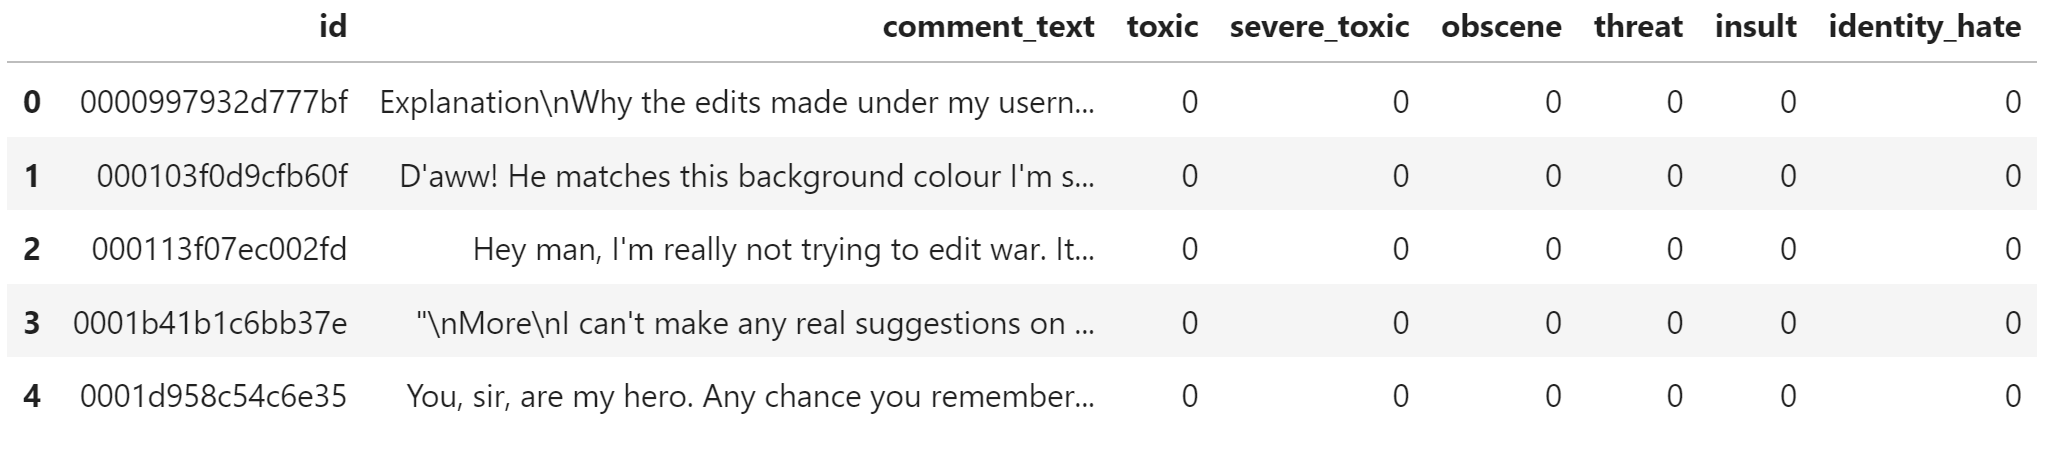
\includegraphics[scale=0.37]{dataset_example.png}
\captionof{table}{Example of data from the Kaggle dataset}
\label{tab_dataset}
\end{center}

\vspace{0.3cm}
\begin{multicols*}{2}

\newpage
\section{Dataset}
The task of toxic comment classification lacks a  consistently labeled standard dataset for comparative evaluation (Schmidt and Wiegand, 2017) \cite{SchmidtandWiegand}.  While there are a number of annotated public datasets in adjacent fields, such as hate  speech (Ross et al., 2016; Gao and Huang,  2017) \cite{RossHuang}, racism/sexism (Waseem, 2016; Waseem  and Hovy, 2016) \cite{HateSpeechDetection} or harassment (Golbeck et al.,  2017) \cite{OnlineHarassmentResearch} detection, most of them follow different definitions for labeling and therefore often constitute  different problems.\\

\begin{center}
\centering % centering table
\begin{tabularx}{0.4\textwidth}{YY} % creating eight columns
\hline\hline %inserting double-line
Class &  \# of occurrences \\ 
\hline % inserts single-line
Clean &  201,081 \\ % Entering row contents
Toxic & 15,294 \\
Obscene & 8,449 \\ % Entering row contents
Insult & 7,877 \\
Identity Hate & 1,405 \\ % Entering row contents
Severe Toxic & 1,595 \\
Threat & 478 \\ % [1ex] adds vertical space
\hline % inserts single-line
\end{tabularx}
\captionof{table}{Class distribution of Wikipedia dataset. The distribution shows a strong class imbalance.}
\label{tab_class}
\end{center}
\vspace{0.3cm}

We analyse a dataset published by Google Jigsaw  in December 2017 over the course of the ‘Toxic  Comment Classification Challenge’ on Kaggle \cite{datasetkaggle}. It  includes 223,549 annotated user comments collected from Wikipedia talk pages and is the largest  publicly available for the task. These comments  were annotated by human raters with the six labels  ‘toxic’, ‘severe toxic, ‘insult’, ‘threat’, ‘obscene’  and ‘identity hate’. 


Comments can be associated  with multiple classes at once, which frames the  task as a multi-label classification problem. Jigsaw has not published official definitions for the  six classes. But they do state that they defined a  toxic comment as “a rude, disrespectful, or unreasonable comment that is likely to make you leave  a discussion.

The dataset features show an unbalanced class distribution, shown in Table \ref{tab_dataset} and in Table \ref{tab_class}. 201,081 samples fall under the majority ‘clear’ class matching none of the six categories, whereas 22,468 samples belong to at least one of the other classes. While the ‘toxic’ class includes 9.6\% of the samples, only 0.3\% are labeled as ‘threat’, marking the smallest class.
Comments were collected from the English Wikipedia and are mostly written in English with some outliers, e.g., in Arabic, Chinese or German language. The domain covered is not strictly locatable, due to various article topics being discussed. Still it is possible to apply a simple categorization of comments as follows: 
\begin{enumerate}
  \item ‘community-related’:\\\\\vspace{0.2cm}
  \fbox{\begin{minipage}{19em}
    Example: “If you continue to vandalize \\
    Wikipedia, you will be blocked from editing.”
    \end{minipage}}
  \item ‘article-related’:\\\\\vspace{0.2cm}
  \fbox{\begin{minipage}{19em}
    Example: “Dark Jedi Miraluka from the MidRim world of Katarr, Visas Marr is the lone surviving member of her species.”
    \end{minipage}}
  \item ‘off-topic’:\\\\\vspace{0.2cm}
  \fbox{\begin{minipage}{19em}
    Example: “== I hate how my life goes today == Just kill me now.”
    \end{minipage}}
\end{enumerate}

\section{Experimental setup}
The experiments involve models from scikit-learn and tensorflow libraries.\\
Those from scikit-learn library are: Multinomial Naive Bayes, Linear Support Vector Classifier, Logistic Regression, K-Nearest Neightbours and Multi-layer Perceptron. A tf-idf vectorization, using stopwords from nltk library, of the input sentences are provided as input to all the models. A One-vs-the-rest (OvR) multiclass strategy is used with all the models and it consists in fitting one classifier per class and for each classifier, the class is fitted against all the other classes.\\
Those from tensorflow library are: Deep Echo State Network and distilBERT. The models are built using the keras build-in functions of tensorflow.\\
A grid search was done to find the final hyper-parameters of each model except for distilBERT because of computational and time constraints.

\subsection{Multinomial Naive Bayes}

This model is implemented using the MultinomialNB class that implements the naive Bayes algorithm for multinomially distributed data. The distribution is parametrized by vectors $\theta_{y}=(\theta_{y1},...,\theta_{yn})$ for each class y, where n is the number of features (in text classification, the size of the vocabulary) and $\theta_{y}=P(x_{i}|y)$ of feature $i$ appearing in a sample belonging to class $y$.\\
The parameter $\theta_{y}$ is estimated by a smoothed version of maximum likelihood, i.e. relative frequency counting:

\begin{equation}
\hat\theta_{y}=\frac{N_{yi}+\alpha}{N_{y}+\alpha n}
\end{equation}

where $N_{yi}$ is the number of times feature $i$ appears in a sample of class $y$.\\
With the parameter fit\_prior=True is assumed a uniform prior, with the parameter class\_prior=None the prior is adjusted according to the data \cite{mnb}.

\subsection{Linear Support Vector Classifier}
In a Linear Support Vector Machines we have a training dataset with \textit{n} points of the form $(\boldsymbol{x_{1}}, y_{1}),...,(\boldsymbol{x_{n}},y_{n})$, where the $y_{i}$ are either 1 or $-1$, each indicating the class to which the point $\boldsymbol{x_{i}}$ belongs. Each $\boldsymbol{x_{i}}$ is a  p-dimensional real vector. We want to find the "maximum-margin hyperplane" that divides the group of points $\boldsymbol{x_{i}}$ for which $y_{i}=1$ from the group of points for which $y_{i}=-1$, which is defined so that the distance between the hyperplane and the nearest point $\boldsymbol{x_{i}}$ from either group is maximized. Any hyperplane can be written as the set of points $\boldsymbol{x}$ satisfying $w^{T}x-b=0$, where $\boldsymbol{w}$ is the (not necessarily normalized) normal vector to the hyperplane. $\frac{b}{\lVert w \lVert}$ determines the offset of the hyperplane from the origin along the normal vector $\boldsymbol{w}$ \cite{lsvc}.\\
This model is implemented using the LinearSVC class that implements the Support Vector Classifier with linear kernel. It is capable of performing binary and multi-class classification on a dataset.\\
The parameter class\_weight=balanced to automatically adjust weights inversely proportional to class frequencies in the input data.

\subsection{Logistic Regression}

The Logistic Regression is a simple model described by the equation $\frac{1}{1+e^{-wx}}$, in which we basically learn to binary separate the samples by softening the Perceptron's step-function with the continuous differentiable logistic equation previously described.\\
This models is implemented using the LogisticRegression class that implements regularized logistic regression. The solver is setted to "lbfgs" \cite{LogisticRegression}. 

\subsection{K-Nearest Neighbours}
The K-nearest neighbours is a non-parametric classification method in which the input consists of the k closest training examples in the dataset. The output is a class membership in which an object is classified by a plurality vote of its neighbors, with the object being assigned to the class most common among its k nearest neighbors \cite{KNearestNeightbours}.\\
The model is implemented using the KNeighborsClassifier class that implements the k-nearest neighbors vote.
The number of neighbors is set to 5.

\subsection{Multi-layer Perceptron}
The Multi-layer Perceptron is a layered model made of different layers of artificial neurons, such that each unit receives input only from units in the immediate preceding layer. Each layer has a set of parameters \textbf{W} to be learned through a proper learning algorithm. Each unit computes a weighted sum of its input $net_{j}=\sum_{i=0}^nw_{ij}a_{i}$, where a is the output of the previous layer, and then it applies an activation function \textit{f} (e.g: sigmoid) such that the output $a_{j}=f(net_{j})$. \cite{Multilayer}\\
This model is implemented using the MLPClassifier class that optimizes the log-loss function. The solver used is "Adam", with one hidden layer with 100 units and "ReLu" activation function. The learning rate is setted to "0.001" with a maximum iterations of 100.

\subsection{Deep Echo State Network}

The Echo State Network is a Reservoir Computing approach that uses a Recurrent Neural Network (RNN) with a sparsely connected hidden layer named "reservoir" with fixed and randomly assigned weights. The reservoir is constructed in such a way that respect the Echo State Property (ESP) that guarantees asymptotic stability to the reservoir in a dynamical system perspective; practically the recurrent weight matrix of the reservoir is scaled with the desired spectral radius, that in theory is 1. The weights of output neurons, called "readout", can be learned so that the network can produce or reproduce specific temporal patterns.\\
This model is implemented using the \href{https://github.com/gallicch/DeepRC-TF/blob/master/DeepRC.py}{DeepRC.py} of Prof. Gallicchio for the reservoir and keras for the readout.\\
The reservoir has 10 layers and each one with 200 units. Each reservoir layer computes the state of the RNN at each time step t as $h(t)=(1-\alpha)h(t-1)+\alpha tanh(\boldsymbol{U}x(t)+\boldsymbol{W}h(t-1))$, where $\boldsymbol{U}$ (with the same dimension of the input) is the input weight matrix, $\boldsymbol{W}$ (with dimension NxN where N is the number of recurrent units) is the recurrent weight matrix and $\alpha$ is the leaking rate ($\alpha \in (0,1]$). In a multi-layer setting, the output of a reservoir layer is the input of the next reservoir layer \cite{gallicchio2017deep}.\\
The readout take as input the output of the reservoir and is made by 2 dense layers with, respectively, 100 and 50 units and "ReLu" activation function with two dropout layers after each dense layer. The output is a dense layer with 6 units (as the number of labels) and "sigmoid" as activation function.\\
The model is optimized minimizing the binary crossentropy using "Adam" as optimizer with a learning rate of "0.001". The total number of trainable parameters are 25,456 and the number of epochs used for the training is 1.\\
A tf-idf vectorization of the inputs are provided to the model using 10 most common words.

\subsection{DistilBERT}

The distillation is a compression technique in which a compact model, the student, is trained to reproduce the behaviour of a larger model, the teacher, or an ensemble of models, in some sense it is similar to a posterior approximation.\\
Bert ("bert-base") is an encoder-decoder network. Both encoder and decoder sections of transformer are a stack of 6 identical layers of multi-head attention and feed forward sublayers with 768 hidden units. The decoder has an additional sublayer which performs attention over output.\\
DistilBERT is a small, fast, cheap and light Transformer model trained by distilling BERT base. It has 40\% less parameters than "bert-base-uncased", runs 60\% faster while preserving over 95\% of BERT’s performances. It does not have token-type embeddings, pooler and retains only half of the layers of BERT and it has 66M parameters \cite{sanh2019distilbert}.\\
The model is implemented using TFDistilBertModel based on "distilbert-base-uncased" of huggingface library. The output of the [CLS] token is fed in input to a dense layer with 50 units and "ReLu" activation function, a dropout of the 10\% and finally to a dense layer of 6 units (as the number of labels) with a "sigmoid" activation function.\\
The model is optimized minimizing the binary crossentropy using "Adam" as optimizer.\\
There are two versions of the model: the one with distilBERT layer with non trainable and fixed weights with only 38,756 trainable parameters over 66,401,636 and the other with distilBERT finetuned with 66,401,636 trainable parameters.\\
The first model is trained for 4 epochs, instead for the second have been used 2 epochs.\\
It is used the class DistilBertTokenizerFast of huggingface for the tokenization of the inputs. The inputs are passed in batches to the model and accepts also the attention mask of the corresponding inputs. The input sequences has a maximum length of 100.

\section{Results and discussion}

\begin{center}
\captionof{figure}{Average percentage of classes per label.}
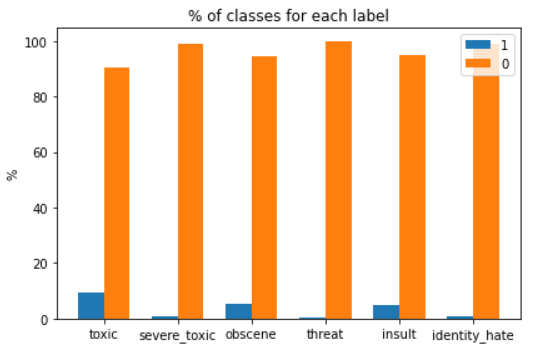
\includegraphics[scale=0.28]{avg_class_per_label.png}
\label{tab_avg_class}
\end{center}

AUC score uses True Positive Rate (TPR or Recall) and False Positive Rate (FPR). Precision-Recall analysis, on the other hand, exchanges FPR for Precision. Then, while AUC uses all the cells (TP, FP, TN, FN) of the Confusion Matrix, Precision-Recall disregards the True Negatives, which have a high impact on an imbalanced problem, since almost all of the data is of the negative class. Therefore, Precision-Recall gives more weight to the majority class (the negative class) than the AUC. This is why the AUC is more suitable for heavily imbalanced problems \cite{MetricsforImbalanced} \cite{ROCCurvesImbalancedClassification}.\\
The best model  is the Logistic Regression with an AUC score of "0.9734" far from the Kaggle SOTA AUC of "0.9885" and a low accuracy of "0.8130" that is not significant for this task as stated before.\\
The second best model is distilBERT with an AUC score of "0.9411" and an accuracy of "0.9713".\\
Overall the two models are slightly similar w.r.t. F1 score.

\end{multicols*}



\begin{center}
\centering
\begin{tabularx}{\textwidth}{Y |YYYYY|Y}

\hline\hline \\

\textbf{Model} & \textbf{P} & \textbf{R} & \textbf{F1} & \textbf{AUC} & \textbf{Accuracy} & {} \vspace{0.2cm} \\
    
\hline\\

\textbf{Multino-mialNB} & 0.90 & 0.11 & 0.19 & 0.8482 & 0.8986 & \textbf{VL} \\
 & 0.84 & 0.12 & 0.20 & 0.8482 & 0.8986 & \textbf{TS} \vspace{0.1cm}\\
 
\hline\\

\textbf{LinearSVC} & 0.67 & 0.77 & 0.72 & 0.8263 & 0.8950 & \textbf{VL} \\
 & 0.47 & 0.81 & 0.59 & 0.8429 & 0.8325 & \textbf{TS} \vspace{0.1cm}\\
 
\hline\\

\textbf{Logistic Regression} & 0.61 & 0.85 & 0.70 & 0.9782 & 0.88 & \textbf{VL} \\
 & 0.42 & 0.88 & 0.56 & \cellcolor{lightgray}0.9734 & 0.8130 & \textbf{TS} \vspace{0.1cm}\\

\hline\\

\textbf{KNeighbors Classifier} & 0.81 & 0.17 & 0.27 & 0.5710 & 0.9012 & \textbf{VL} \\
 & 0.63 & 0.18 & 0.28 & 0.5729 & 0.8999 & \textbf{TS} \vspace{0.1cm}\\

\hline\\

\textbf{MLP-Classifier} & 0.73 & 0.66 & 0.69 & 0.9594 & 0.9001 & \textbf{VL} \\
 & 0.54 & 0.69 & 0.60 & 0.9564 & 0.8524 & \textbf{TS} \vspace{0.1cm}\\ 

\hline\\

\textbf{DeepESN} & 0.21 & 0.01 & 0.01 & 0.7145 & 0.9629 & \textbf{VL} \\
 & 0.17 & 0.00 & 0.01 & 0.6779 & 0.9621 & \textbf{TS} \vspace{0.1cm}\\ 

\hline\\

\textbf{distilBERT} & 0.82 & 0.54 & 0.64 & 0.9567 & 0.9790 & \textbf{VL} \\
 & 0.65 & 0.51 & 0.56 & 0.9411 & \cellcolor{lightgray}0.9713 & \textbf{TS} \vspace{0.1cm}\\ 

\hline\\

\textbf{distilBERT (finetuned)} & 0.84 & 0.54 & 0.65 & 0.9544 & 0.9790 & \textbf{VL} \\
 & 0.66 & 0.52 & 0.57 & 0.9403 & 0.9711 & \textbf{TS} \vspace{0.1cm}\\ 

\hline\\

\end{tabularx}
\captionof{table}{Validation and Test scores (Kaggle SOTA AUC: 0.9885).}
\label{tab_val_scores}
\end{center}
\vspace{0.3cm}


\begin{multicols*}{2}

\section{Conclusion}
This task was very challenging in terms of training a model on sparse toxic comments.\\
It was a surprise to notice how a simple model in a OvR setting performs better than complex models as distilBERT.\\
Probably a model selection phase and the using of more epochs should increase the performances of distilBERT, but training a transformer is heavy and requires a lot of time.\\
In our opinion the models performances are far from the State of the Art because of the imbalanced dataset, as shown in Figure \ref{tab_avg_class}, that led to have low value of P/R and F1 scores.\\

As a future work, 5 experiments could be done to handle unbalanced data as follows:
\begin{enumerate}
    \item Define higher weight for label ‘1’: Depending on how imbalanced the data is, we put higher weight on the minority label to force the classifier to work harder on label ‘1’. For example, if the ratio of label ‘1’ to the label ‘0’ is 1:9 we will put 0.9 as the weight factor on label ‘1’.
    \item Over-sampling label ‘1’ (minority class): To reduce the imbalance, we simply duplicate samples with label ‘1’ to achieve 1:1 as the ratio of negative samples to positive samples. But there is a downfall for this method. It might result in over-fitting.
    \item Under-sampling label ‘0’ (majority class): To reduce the imbalance, this time we reduce the number of negative samples with label ‘0’ to get the ratio of negative samples to positive samples closer to 1:1. This also has a disadvantage of losing potentially important data.
    \item Performing dataset augmentation.
    \item Performing stratified sampling during training.
\end{enumerate}


\bibliographystyle{plain}
\bibliography{sample.bib}

\end{multicols*}
\end{document}